\chapter{Funkcja celu -- porównanie barwy dźwięku} \label{target_function_chapter}

Aby stopniowo dostosować graf przetwarzania sygnałów zaimplementowany 
w rozdziale~\ref{dsp_graph_chapter} do imitowania zadanej próbki dźwięku,
należy wykorzystać funkcję celu, która maleje wraz ze wzrostem podobieństwa
barwy dźwięku między próbki zadaną i sygnałem generowanym przez graf. 

\begin{figure}[H]
    \centering
    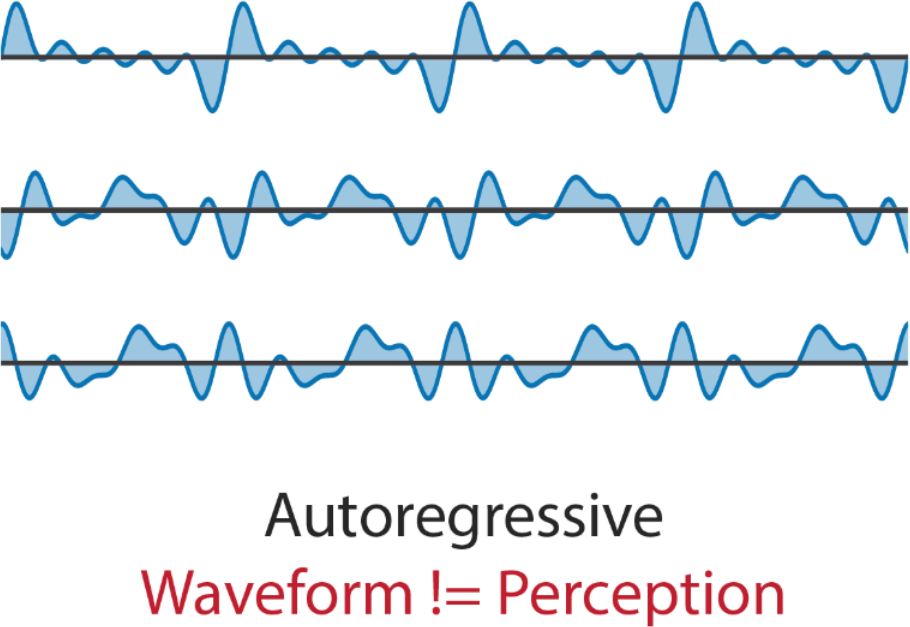
\includegraphics[width=0.5\linewidth]{rys03/d_dsp_example_graph.png}
    \caption{
      Przykład trzech próbek dźwięku, które dla słuchacza brzmią identycznie, mimo
      znacznych różnic w kształcie fali. Źródło obrazka: \cite{engel2020ddsp}.
    }
    \label{fig:waveform_not_equal_to_perception}
\end{figure}

\section{Porównanie barwy dźwięku w literaturze} \label{sec:timbre_comparison_literature_overview}

Żadna z prac przeanalizowanych podczas przeglądu literatury
(\cite{engel2020ddsp}, \cite{ieee_synth_programming}, \cite{ddx7}, \cite{riffusion},
\cite{evolutionary_puredata}, \cite{parallel_evolutionary_optimization_synth_parameters}, \cite{mfcc_dtw})
nie wykorzystuje metod porównywania sygnału osadzonych jedynie w dziedzinie czasu, ponieważ
nie są one skuteczne do porównywania dźwięków pod względem odczuć psychoakustycznych.
Przykład różnych kształtów fali, które z perspektywy słuchacza brzmią jak
taki sam dźwięk zademonstrowano na rysunku~\ref{fig:waveform_not_equal_to_perception}.

Ponieważ porównywanie barwy dźwięku instrumentów muzycznych nie należy do popularnych
tematów badań, podczas przeglądu literatury wykorzystano również badania dotyczące
rozpoznawania głosu, wykorzystujące współczynniki MFCC oraz
\textit{dynamic time warping} \cite{mfcc_dtw}.

\subsection{Analiza metod z literatury}

Metody zaczerpięte z literatury wykorzystują różne podejścia do funkcji celu.
Podejścia te można usystematyzować za pomocą dwóch cech:

\begin{enumerate}
  \item Rodzaj wykonanej transformacji do dziedziny częstotliwości:
  \begin{itemize}
    \item MFCC \cite{ieee_synth_programming} \cite{evolutionary_puredata} \cite{mfcc_dtw},
    \item Transformata Fouriera (w różnych konfiguracjach) \cite{riffusion} \cite{ddx7}.
  \end{itemize}
  \item Dalsze przetwarzanie sygnału mające ułatwić optymalizację:
    \begin{itemize}
      \item Ustawianie wagi konkretnym próbkom na podstawie metryki określającej siłę sygnału
        (na przykład \textit{root-mean-square})
        \cite{parallel_evolutionary_optimization_synth_parameters},
        aby wzmocnić istotność głośniejszych fragmentów dźwięku,
      \item Wykorzystanie \textit{dynamic time warping}, aby funkcja celu przyzwalała na
        niedokładności w odwzorowaniu dokładnej prędkości zmian w charakterystyce spektralnej \cite{mfcc_dtw}.
    \end{itemize}
\end{enumerate}


